\section{Memory-augmented Online VAD}
\label{sec:theory}

\fboxsep=1mm%padding thickness
\fboxrule=1pt%border thickness

\begin{figure}[!t]
            \centerline{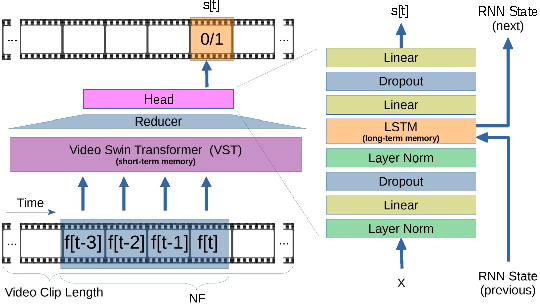
\includegraphics[clip, width=\linewidth]{images/arch-rx-cropped.pdf}}
        \caption{The online frame-level Video Anomaly Detection (VAD) architecture. $f[t]$ is the frame at time $t$, $x$ the output of the Reducer, $\mathit{NF}$ the number of frames in input to the VST, $s[t]$ the anomaly classification score of the frame $f[t]$.\label{fig:arch}}
\end{figure}

In this section the MOVAD architecture is described.  
The model is composed by: a short-term memory module and a classification head that includes a long-term memory module (see Fig.~\ref{fig:arch}). 
Taking inspiration from~\cite{xu2021long}, recently observed frames have been taken into account as a source of information related to the ongoing action, and past frames to take into account the context.

\noindent\textbf{Short-term memory module.}
Since we are dealing with the online version of VAD task, the only information available to the system, at any given time, are the current and the past frames.
In order to implement this module, we selected the Video Swin Transformer (VST)~\cite{liu_video_2022} over ViViT~\cite{Arnab_2021_ICCV} due to its superior performance, and over an RNN given its ability to process frames in parallel.
Originally born to carry out the Video Action Classification task analyzing all the frames in one step, we adapted to perform single-frame classification using few of them.
In particular, it considers only a small temporal window of $\mathit{NF}$ frames of the video, going from the current frame at time $t$ to the previous frames at time $t-\left(\mathit{NF}-1\right)$.
VST takes as input a video with size $\mathit{NF} \times H \times W \times 3$, where $\mathit{NF = 4}$, $H$ e $W$ correspond to the number of frames, height, width and RGB channels, respectively.
The model internally splits the frames in non-overlapping 3D patches, partitioning the video in $\frac{\mathit{NF}}{2} \times \frac{H}{4} \times \frac{W}{4}$ 3D tokens, projecting the features to an arbitrary dimension $C$.
The rest of the architecture is similar to the original Swin Transformer~\cite{liu2021Swin}, with four stages of Video Swin Transformer blocks, interspersed with $2\times$ spatial down-sampling in the patch merging layer.

\noindent\textbf{Long-term memory module.}
The output of VST goes through Adaptive Average Pool 3D layer (Reducer in Fig.~\ref{fig:arch}) and, finally, enter inside the classification Head.
As shown in Fig.~\ref{fig:arch}, the Head is composed by a series of normalization layers, linear layers and dropout, alternating. 
It deals with long-term memory thanks to a LSTM module inserted after the last normalization layer.
This module is composed by three cells stacked together to form a stacked LSTM.
The state, composed by an hidden state $h_t$ and cell state $c_t$, is updated whenever a new frame is analyzed.
The LSTM receives in input a features block of $[B, 1024]$, where $B$ is the batch size, and returns a block of same size together with the state of cells.
Because the state is relatively small, the module is very efficient and leads to a fixed and limited additional computational cost.
For each frame $f[t]$, the model outputs the anomaly classification score $s_t \in [0,1]$, where $0$ means no anomaly and $1$ means the frame is anomalous.
A weighted cross-entropy loss was chosen the model, giving higher weight to the anomaly class, in order to reflect the distribution of the data.

% copyright image frame: <a href="https://www.freepik.com/free-vector/realistic-vector-icon-film-tape-strip-with-white-square-isolated-white-cinema-concept_31096470.htm#query=video%20frame&position=31&from_view=keyword">Image by user15245033</a> on Freepik